\chapter{Modulation}

\section{Introduction}
Modulation is done when message signal is not capable of propagating long distance, we change the signal by multiplying another high frequency signal and send the modulated signal.

\par The characteristics of the message signal, if changed, the message contained in it also alters. Hence, it is a must to take care of the message signal. A high frequency signal can travel up to a longer distance, without getting affected by external disturbances. We take the help of such high frequency signal which is called as a carrier signal to transmit our message signal. Such a process is simply called as Modulation.

Modulation is the process of changing the parameters of the carrier signal, in accordance with the instantaneous values of the modulating signal.

\section{Advantages of Modulation}
The antenna used for transmission, had to be very large, if modulation was not introduced. The range of communication gets limited as the wave cannot travel a distance without getting distorted.

Following are some of the advantages for implementing modulation in the communication systems.

\begin{itemize}
  \item Reduction of antenna size
  \item No signal mixing
  \item Increased communication range
  \item Multiplexing of signals
  \item Possibility of bandwidth adjustments
  \item Improved reception quality

\end{itemize}

\section{Types of Modulation}
There are many types of modulations. Depending upon the modulation techniques used, they are classified as shown in the following figure.
\subfile{Lectures/types.tex}

\chapter{Amplitude Modulation}
In continuous-wave modulation, a high frequency sine wave is used as a carrier wave. This is further divided into two types

\begin{enumerate}
  \item Amplitude Modulation
  \item Angle Modulation
\end{enumerate}

\section{Amplitude Modulation (AM)}
In analog modulation, the amplitude of the carrier signal is made to follow that of the modulating signal. Several variants of amplitude modulation are used in practice. They are Double Side Band Suppressed Carrier (DSBSC) Modulation, Single Sideband Suppressed Carrier (SSBSC) Modulation and Vestigial Sideband Amplitude Modulation (VSBAM).

\subsection{Introduction}
Let m(t) denote a signal that contains information to be transmitted. The information can
take analog form or digital form. In traditional analog radio broadcast, m(t) would be an audio
signal. In digital communication systems, m(t) may be a sequence of pulses that carries binary
data. The information-bearing signal m(t) will be called a message signal for convenience. Also,
we will assume that m(t) is a baseband signal with bandwidth W Hz.
In baseband transmission systems such as wireline telephone systems, we may directly transmit
m(t). However, there are many scenarios where the physical medium or channel is bandpass.
In particular, in wireless communications, a channel operates over a certain frequency range (or
frequency band); the operating frequencies are from 30 kHz and upward. In such scenarios, it would
be appropriate to consider carrier modulation. Let

\begin{equation*}
  c(t) = A_c cos(2\pi f_c t + \phi)
\end{equation*}
denote a sinusoidal carrier wave, where A c is the carrier amplitude and f c is the carrier frequency.
We wish to use the carrier wave to carry the message signal, so that the message signal can
appropriately be transmitted over a bandpass channel.
There are various carrier modulation techniques. Among them, amplitude modulation (AM) is
considered the oldest. This handout considers AM.

\subsection{Baseband \& Carrier communication}
\begin{enumerate}
  \item Baseband communication\\
  \begin{itemize}
    \item No Shift in the range of frequencies
    \item FDM
  \end{itemize}

  \item Carrier communication\\
  \begin{itemize}
    \item Uses modulation to shift frequency spectrun
    \item Three parts of a carrier
  \end{itemize}

\end{enumerate}

\subsection{Amplitude Modulation Principle}
The amplitude-modulated wave may be described by the following formula
\begin{equation}
  s(t) = [1 + k a m(t)] c(t)\\
  = A c [1 + k a m(t)] cos(2\pi f_c t),
\end{equation}
where k a is a constant and is called the amplitude sensitivity. Figures 1.(a)-(b) gives an illustration
of the AM process. In the illustration of the AM wave in Figure 1(b), the constant k a is adjusted
such that $1 + k a m(t) \geq 0$ for all t. It is observed that the envelope of the AM wave takes the same
shape as the message signal (more precisely, the waveform 1 + k a m(t)). In fact, the idea of AM is
to use the envelope of the modulated wave s(t) to carry the message signal.
There is a requirement for AM to operate properly. Specifically, we must have
\begin{equation}
  |k a m(t)| \leq 1, for all t.
\end{equation}
The condition in (3) implies that $1 + k a m(t) \geq 0$ for all t. Figure 1.(c) shows a situation where
1 + k a m(t) < 0 for some t. We see that the envelope of the AM wave now becomes a distorted version of the message signal. This phenomenon is sometimes known as overmodulation, which can
happen when k a is set too large.

\begin{figure}[h!]
  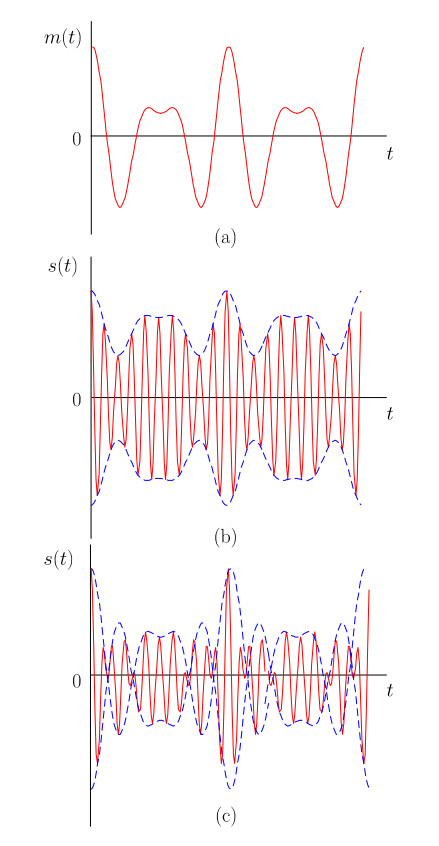
\includegraphics[\textwidth=0.5pt]{figures/AMgraph.png}
  \caption{An illustration of the AM process. (a) The message signal m(t). (b) The AM wave s(t)
when $|k a m(t)| \leq 1$ holds for all t. (b) The AM wave s(t) when we have |k a m(t)| > 1 for some t.}
  \label{fig:f2}
\end{figure}


We consider several modifications of the previously studied AM scheme, namely, double sideband-
suppressed carrier modulation, single sideband modulation and quadrature amplitude modulation.

While the AM scheme is rarely seen in modern communication, we still see some AM concepts,particularly quadrature amplitude modulation, being used—that includes advanced digital com-
munication systems.


\chapter{Double Side-Band Suppressed Carrier}
Recall that m(t) denotes the message signal, and $c(t) = A_c cos(2 \pi f_ct)$ denotes the sinusoidal carrier
wave. Also recall that m(t) is assumed to be a baseband signal with bandwidth W Hz. In double
sideband-suppressed carrier (DSB-SC) modulation, the modulated wave is given by
\begin{equation}
  s(t) = m(t) · c(t)\\
  = A_cm(t) cos(2\pi f_c t)

\end{equation}
The difference between AM and DSB-SC modulation is that the DSB-SC modulated wave does not
have the pure carrier component. Consequently, one hundred percent of the transmission power is
spent on sending the message signal. The Fourier transform of the DSB-SC modulated signal s(t)
is simply
\begin{equation}
  S(f) = \frac{A_c}{2}[M(f − f_c ) + M(f + f_c )]
\end{equation}

Figure 1 illustrates the corresponding amplitude spectrum. As can be seen in the figure, the
transmission bandwidth of DSB-SC modulation is 2W Hz—the same as the AM transmission
bandwidth.


The modulation process of DSB-SC modulation is similar to that of AM. Figure 2 shows a
DSB-SC modulation process via the product modulator.
